\chapter{Bildverarbeitung}

Die Bildverarbeitung besteht im Wesentlichen aus der Generierung von einzelnen Videoframes im RGB565 – Bitmap Format, welche optisch den Anforderungen aus \textbf{Kapitel X} entsprechen müssen. Die einzelnen Videoframes werden von der Schnittstelle \textbf{IFrameProvider} empfangen und nach der Verarbeitung an die Schnittstelle \textbf{FrameViewer} zur Darstellung auf dem Display des Smartphones weitergereicht.
\\
\\
Im ersten Ansatz, der verfolgt wurde, benötigte es eine Konvertierung als Vorverarbeitung der einzelnen Frames in den RGB Farbraum (siehe Kapitel \ref{YUV_RGBKonvert}). Diese Vorverarbeitung wurde im späteren Verlauf überflüssig, da das Übertragungsformat der Videoframes aufgrund der in \textbf{Kapitel X} aufgelisteten Gründen geändert wurde. Der Vollständigkeit halber wird eben genannte Konvertierung hier trotzdem erläutert.
\\
\\
Es wurde davon ausgegangen, dass die Schnittstelle \textbf{IFrameProcessor} Byte-Streams im Format NV12 (YUV420) erhält, welche zur weiteren Verarbeitung zunächst in den RGB Farbraum überführt werden mussten, um dann als Bitmap-Objekte weiterverarbeitet werden zu können. Die NV12 Byte-Streams liegen im YUV-Farbmodell (siehe Kapitel \ref{YUV_RGBKonvert}) vor. 
\\
\\
Die Methode convertNv12ToBmp(...) (siehe Abbildung \ref{fig:NV12_to_BMP})nimmt ein eindimensionales Byte-Array, welches ein Frame im NV12-Format repräsentiert, entgegen. Die Methode benötigt zusätzlich noch die Höhe und Breite des Frames in Pixeln, um die Positionen der für ein Ausgabepixel relevanten Y, U und V Werte im Array bestimmen zu können. Innerhalb der for-Schleife werden für jedes einzelne Ergebnis-Pixel die in Kapitel \ref{YUV} Luminanz- und Chrominanz-Werte aus dem Array ermittelt und an die Methode convertYUVtoRGB(...) übergeben. Ergebnis dieser Methode ist ein Array aus Integer-Werten, welche jeweils die Farbe eines Pixels repräsentieren. Mit Hilfe dieses Arrays kann anschließend mit der Methode createBitmap(...) der Klasse Bitmap aus dem Android SDK ein Bitmap-Objekt erzeugt werden. 
\clearpage
\begin{figure}[h]
	\centering
	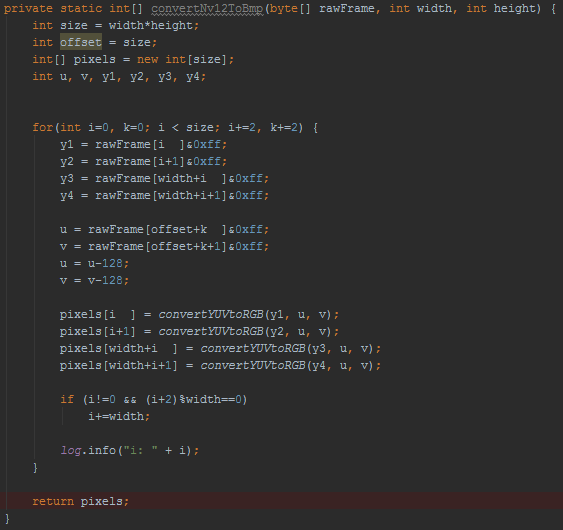
\includegraphics[width=0.9\textwidth]{Bilder/Bildverarbeitung/NV12_to_BMP.PNG}
	\caption{Methode zur Überführung eines Byte-Arrays im NV12-Format in ein Bitmap-Objekt}
	\label{fig:NV12_to_BMP}
\end{figure}

~\\
Die in Abbildung \ref{fig:YUV_to_RGB} gezeigte Methode convertYUVtoRGB(...) übernimmt gemäß der Formeln aus Kapitel \ref{YUV_RGBKonvert} die Berechnung der R, G und B Werte eines Pixels des Ergebnis-Frames. Aus diesen drei Werten wird anschließen ein Integer berechnet, welcher dann allein die Farbe des Pixels repräsentiert.
\clearpage
\begin{figure}[h]
	\centering
	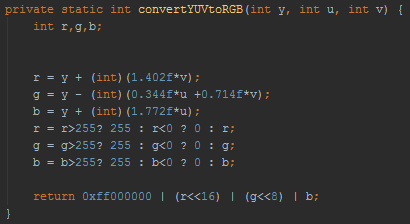
\includegraphics[width=0.7\textwidth]{Bilder/Bildverarbeitung/convert_1_Pixel.PNG}
	\caption{Methode zur Umrechnung eines Pixels aus dem YUV-Farbraum in den RGB-Farbraum}
	\label{fig:YUV_to_RGB}
\end{figure}
